\documentclass[xcolor={table}]{beamer}
\usetheme{Singapore}
\usepackage[utf8]{inputenc}
\usecolortheme{crane}
\usepackage{graphicx}
\usepackage{iwona}
\usepackage{standalone}
\usepackage{tikz}
\usetikzlibrary{arrows}
\usetikzlibrary{decorations.markings}
\usetikzlibrary{calc}
\usetikzlibrary{shapes,snakes}
\usepackage{amsmath}
\usepackage{amsfonts}
\usepackage{amsthm}
\usepackage{mathtools}
\usepackage{minted}
\usemintedstyle{trac}

\definecolor{lightblue}{RGB}{124,190,255}
\definecolor{darkgreen}{RGB}{24,145,0}

\beamertemplatenavigationsymbolsempty
\setbeamerfont{caption}{size=\tiny}


\title{Overview of PhD Work}
\author{Geraint Palmer\newline \scriptsize{Paul Harper, Vincent Knight}}
\date{16\textsuperscript{th} August 2016}
\titlegraphic{
\includegraphics[width=1.5cm]{../cflogo.pdf}}

\begin{document}
\frame{\titlepage}

\begin{frame}
\frametitle{What is a Queue?}
\begin{figure}
  \includestandalone[width=0.8\textwidth]{1nodeexample}
\end{figure}
\end{frame}

\begin{frame}
\frametitle{What is a Queue?}
\begin{figure}
  \includestandalone[width=0.8\textwidth]{2nodefeedbackexample}
\end{figure}
\end{frame}


\begin{frame}
\frametitle{Simulation with Ciw}
\begin{center}
Open Source Python Library\\
\begin{figure}

\includegraphics[width=0.4\textwidth]{logo}
\end{figure}
{\tiny
\href{https://twitter.com/CiwPython}{@CiwPython}\\
\url{https://github.com/geraintpalmer/Ciw}\\
\url{https://pypi.python.org/pypi/Ciw}\\
\url{http://ciw.readthedocs.io}\\}
\end{center}
\end{frame}

\begin{frame}
\begin{columns}
\column{0.03\textwidth}

\column{0.98\textwidth} 
\fontsize{8pt}{10pt} \inputminted{python}{ciwexample_implement.py}
\end{columns}
\end{frame}

\begin{frame}
\frametitle{Visualising Ciw Data}
\begin{center}
\huge{CiwVis}\\
\tiny{\url{https://github.com/CiwPython/CiwVis}}\\

\end{center}
\end{frame}

\begin{frame}
    \frametitle{Deadlock}
    \begin{figure}
    \includestandalone[width=0.7\textwidth]{gridlock}
    \end{figure}
\end{frame}

\begin{frame}
    \begin{figure}
    \includestandalone[width=\textwidth]{buildupdigraph}
    \end{figure}
\end{frame}

\begin{frame}
    \frametitle{Markovian Model of Deadlock}
    \includestandalone[width=\textwidth]{2nodemultiserver}\newline
    \center{\LARGE{$(i, j)$}}
\end{frame}


\begin{frame}
\center
\scriptsize \[S = \{(i,j)\in\mathbb{N}^{(n_1+c_1+c_2)\times (n_2+c_2+c_1)} \nonscript\; | \nonscript\; i \leq n_1+c_1+j, \nonscript\; j \leq n_2+c_2+i\}\]

\scalebox{0.8}{\parbox{.5\linewidth}{%
\begin{align*}
  \delta &= (i_2, j_2) - (i_1, j_1)\\
  b_1 &= \max(0, i_1-n_1-c_1)\\
  b_2 &= \max(0, i_2-n_2-c_2)\\
  s_1 &= \min(i_1, c_1)-b_2\\
  s_2 &= \min(i_2, c_2)-b_1\\
\end{align*}
}}


\begin{table}
\begin{center}
\resizebox{\textwidth}{!}{
\begin{tabular}{ l | l | l | l |}
  & $j_1 < n_2 + c_2$ & $j_1 = n_2 + c_2$ & $ j_1 > n_2 + c_2$ \\ \hline
  \rotatebox[origin=c]{90}{$i_1 < n_1 + c_1$} & \begin{tabular}{ l } \color{red} $\Lambda_1$ if $\delta = (1, 0)$ \\ \color{orange} $\Lambda_2$ if $\delta = (0, 1)$ \\ \color{darkgreen} $r_{12}s_1\mu_1$ if $\delta = (-1, 1)$ \\ \color{green} $r_{21}s_2\mu_2$ if $\delta = (1, -1)$ \\ \color{blue} $(1-r_{12})s_1\mu_1$ if $\delta = (-1, 0)$ \\ \color{lightblue} $(1-r_{21})s_2\mu_2$ if $\delta = (0, -1)$ \end{tabular} & \begin{tabular}{ l } \color{red} $\Lambda_1$ if $\delta = (1, 0)$ \\ \color{darkgreen} $r_{12}s_1\mu_1$ if $\delta = (0, 1)$ \\ \color{green} $r_{21}s_2\mu_2$ if $\delta = (1, -1)$ \\ \color{blue} $(1-r_{12})s_1\mu_1$ if $\delta = (-1, 0)$ \\ \color{lightblue} $(1-r_{21})s_2\mu_2$ if $\delta = (0, -1)$ \end{tabular} & \begin{tabular}{ l } \color{red} $\Lambda_1$ if $\delta = (1, 0)$ \\ \color{darkgreen} $r_{12}s_1\mu_1$ if $\delta = (0, 1)$ \\ \color{green} $r_{21}s_2\mu_2$ if $\delta = (0, -1)$ \\ \color{blue} $(1-r_{12})s_1\mu_1$ if $\delta = (-1, 0)$ \\ \color{lightblue} $(1-r_{21})s_2\mu_2$ if $\delta = (-1, -1)$ \end{tabular} \\ \hline
  \rotatebox[origin=c]{90}{$i_1 = n_1 + c_1$} & \begin{tabular}{ l } \color{orange} $\Lambda_2$ if $\delta = (0, 1)$ \\ \color{darkgreen} $r_{12}s_1\mu_1$ if $\delta = (-1, 1)$ \\ \color{green} $r_{21}s_2\mu_2$ if $\delta = (1, 0)$ \\ \color{blue} $(1-r_{12})s_1\mu_1$ if $\delta = (-1, 0)$ \\ \color{lightblue} $(1-r_{21})s_2\mu_2$ if $\delta = (0, -1)$ \end{tabular} & \begin{tabular}{ l } \color{darkgreen} $r_{12}s_1\mu_1$ if $\delta = (0, 1)$ \\ \color{green} $r_{21}s_2\mu_2$ if $\delta = (1, 0)$ \\ \color{blue} $(1-r_{12})s_1\mu_1$ if $\delta = (-1, 0)$ \\ \color{lightblue} $(1-r_{21})s_2\mu_2$ if $\delta = (0, -1)$ \end{tabular} & \begin{tabular}{ l } \color{darkgreen} $r_{12}s_1\mu_1$ if $\delta = (0, 1)$ \\ \color{green} $r_{21}s_2\mu_2$ if $\delta = (1, 0)$ \\ \color{blue} $(1-r_{12})s_1\mu_1$ if $\delta = (-1, 0)$ \\ \color{lightblue} $(1-r_{21})s_2\mu_2$ if $\delta = (-1, -1)$ \end{tabular} \\ \hline
  \rotatebox[origin=c]{90}{$i_1 > n_1 + c_1$} & \begin{tabular}{ l } \color{orange} $\Lambda_2$ if $\delta = (0, 1)$ \\ \color{darkgreen} $r_{12}s_1\mu_1$ if $\delta = (-1, 0)$ \\ \color{green} $r_{21}s_2\mu_2$ if $\delta = (1, 0)$ \\ \color{blue} $(1-r_{12})s_1\mu_1$ if $\delta = (-1, -1)$ \\ \color{lightblue} $(1-r_{21})s_2\mu_2$ if $\delta = (0, -1)$ \end{tabular} & \begin{tabular}{ l } \color{darkgreen} $r_{12}s_1\mu_1$ if $\delta = (0, 1)$ \\ \color{green} $r_{21}s_2\mu_2$ if $\delta = (1, 0)$ \\ \color{blue} $(1-r_{12})s_1\mu_1$ if $\delta = (-1, -1)$ \\ \color{lightblue} $(1-r_{21})s_2\mu_2$ if $\delta = (0, -1)$ \end{tabular} & \begin{tabular}{ l } \color{darkgreen} $r_{12}s_1\mu_1$ if $\delta = (0, 1)$ \\ \color{green} $r_{21}s_2\mu_2$ if $\delta = (1, 0)$ \\ \color{blue} $(1-r_{12})s_1\mu_1$ if $\delta = (-\min(b_1+1,b_2+1), -\min(b_1,b_2+1))$ \\ \color{lightblue} $(1-r_{21})s_2\mu_2$ if $\delta = (-\min(b_1+1,b_2), -\min(b_1+1,b_2+1))$ \end{tabular} \\ \hline
\end{tabular}
}
\end{center}
\end{table}
\end{frame}

\begin{frame}
    \begin{figure}
    \includestandalone[width=0.95\textwidth]{MC2nodemultiserv}
    \end{figure}
\end{frame}

\begin{frame}
    \frametitle{Times to Deadlock}
    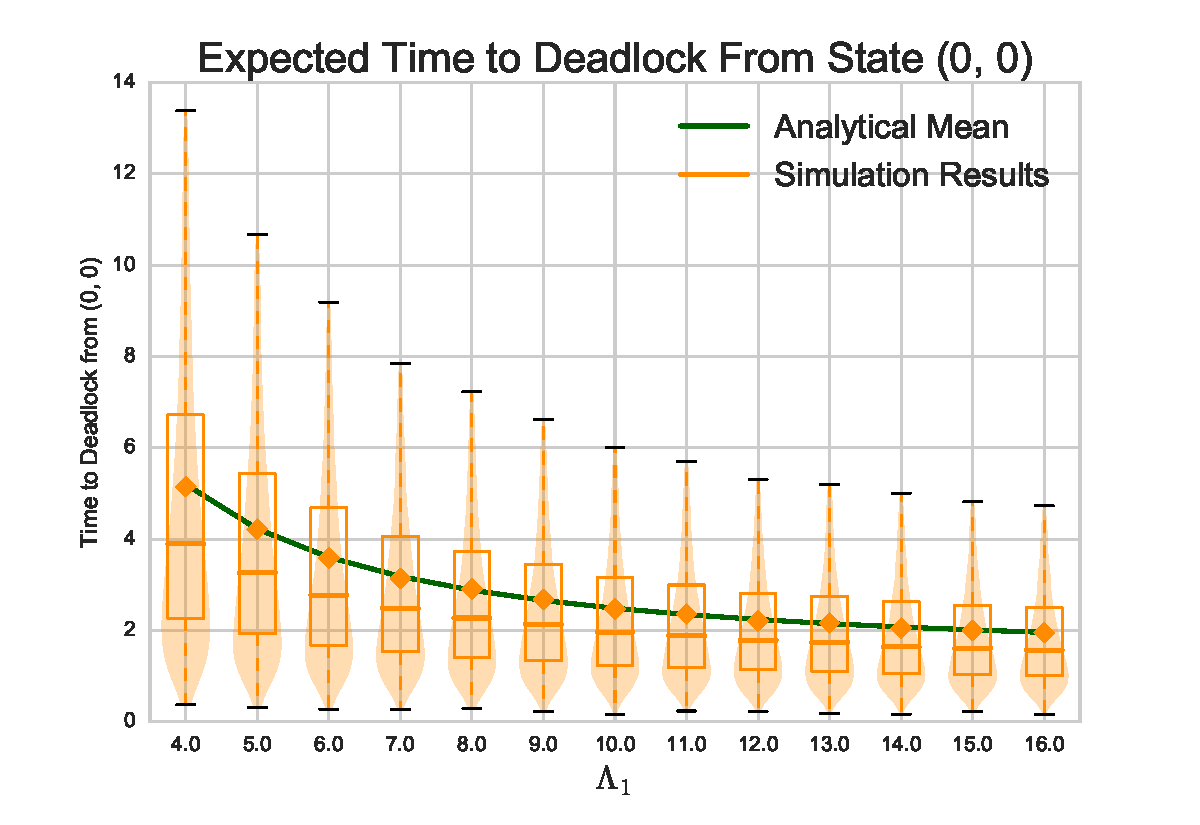
\includegraphics[width=0.5\textwidth]{varyL1_2Nms}
    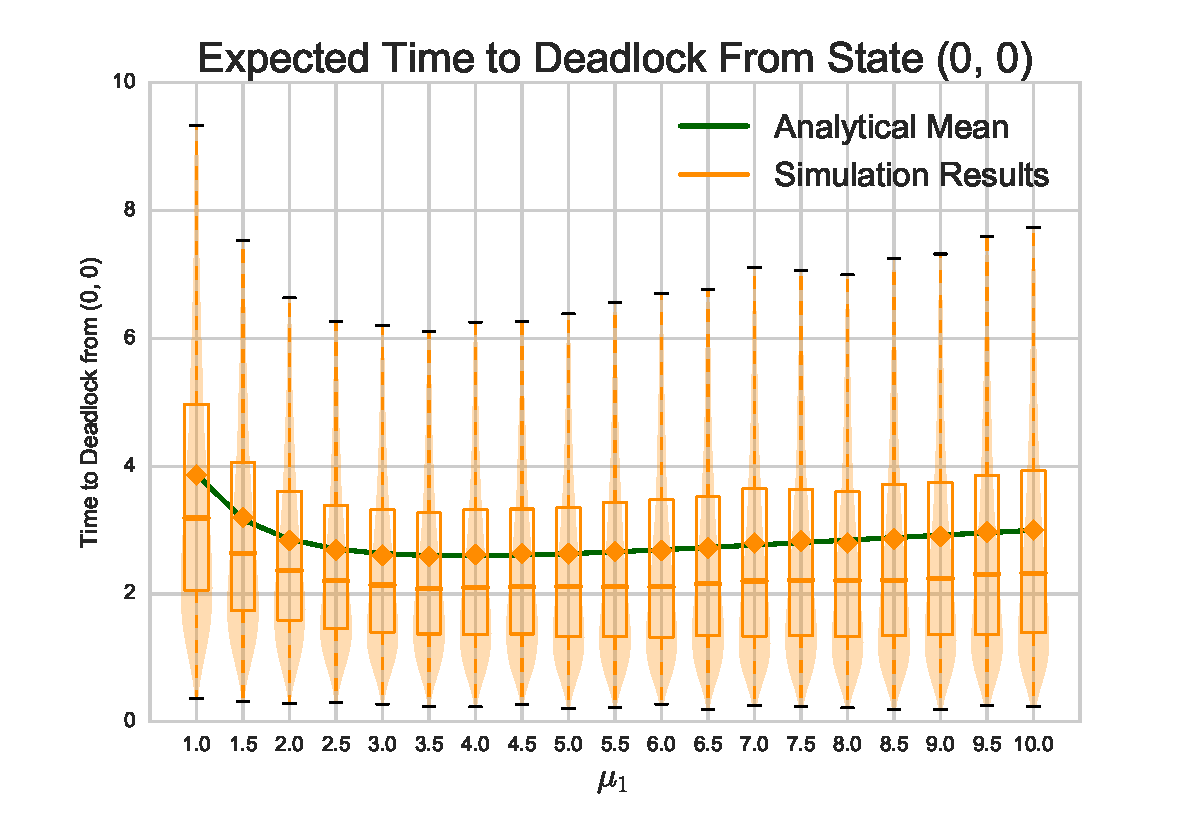
\includegraphics[width=0.5\textwidth]{varymu1_2Nms}\newline
    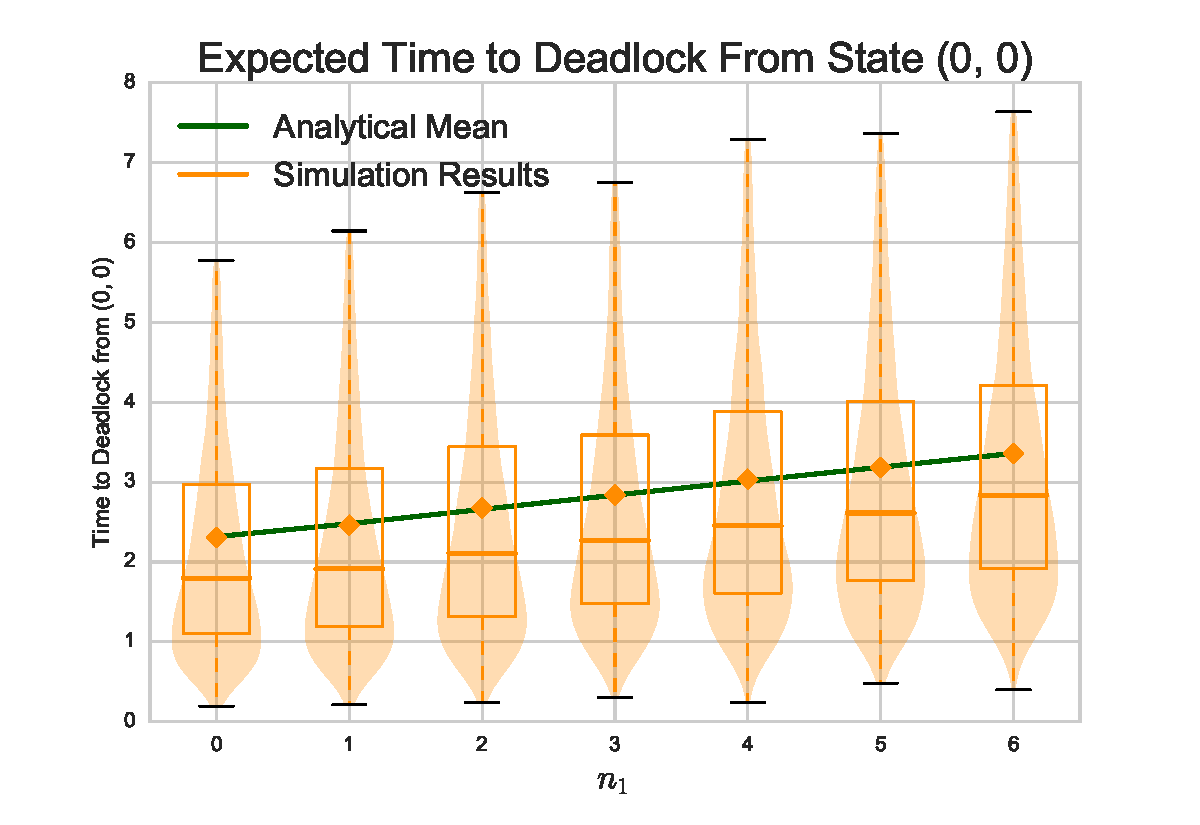
\includegraphics[width=0.5\textwidth]{varyn1_2Nms}
    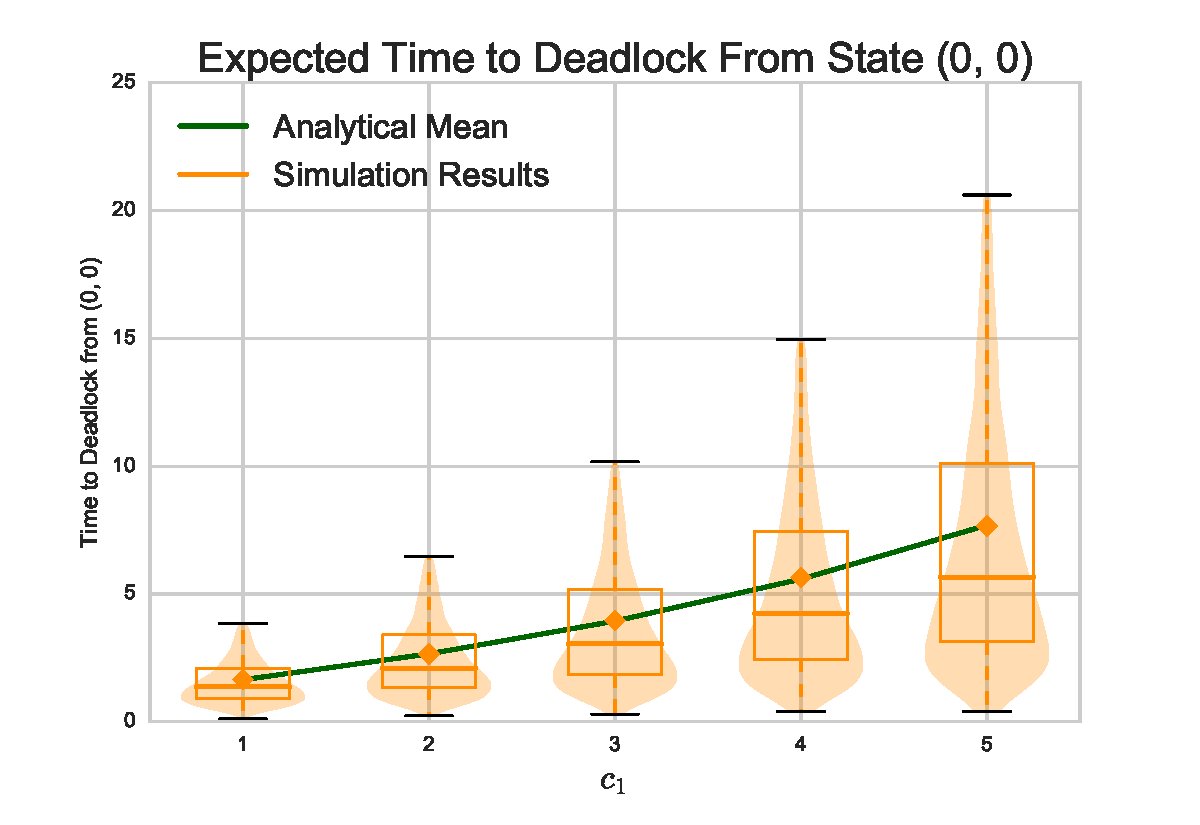
\includegraphics[width=0.5\textwidth]{varyc1_2Nms}
\end{frame}

\begin{frame}
    \frametitle{Optimally Resolving Deadlock}
    \begin{figure}
        \includestandalone[width=0.8\textwidth]{resolution_counterexample}
    \end{figure}
\end{frame}

\begin{frame}
    \frametitle{OPICP}
    \begin{center}
        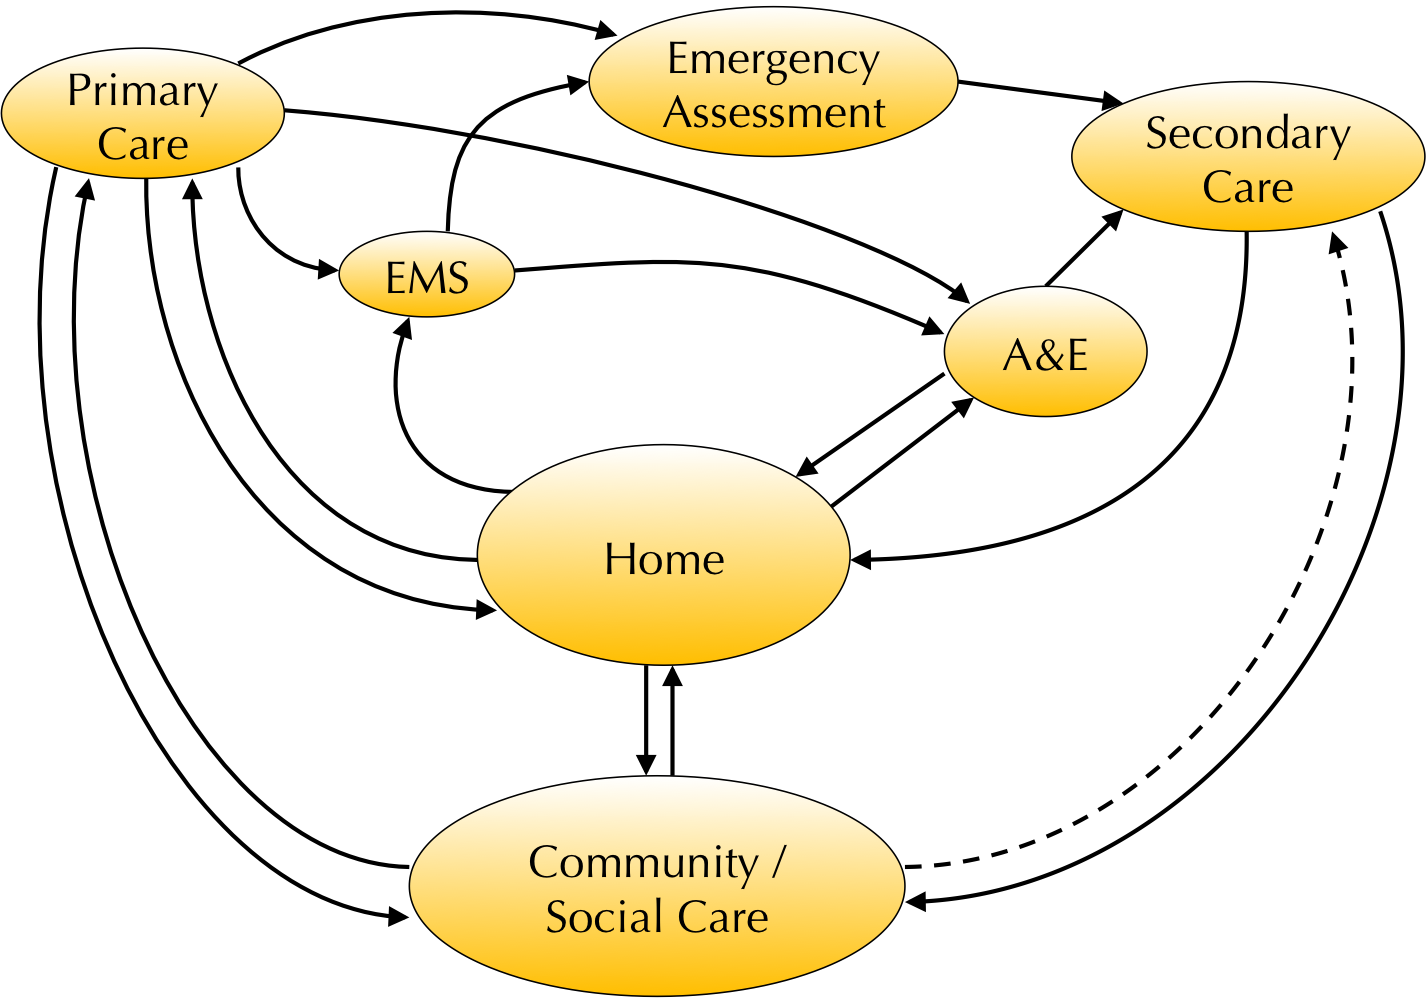
\includegraphics[width=\textwidth]{opicp_concept}
    \end{center}
\end{frame}

\begin{frame}
    \begin{center}
        \huge{Thank you.}
    \end{center}
\end{frame}

\end{document}
